\apendice{Especificación de Requisitos}

\section{Introducción}
En esta sección se presentan los requisitos de la aplicación, abordando tanto los objetivos generales como los específicos del proyecto. Se incluye un catálogo detallado de los requisitos funcionales y no funcionales, que definen el comportamiento y las características técnicas de la aplicación. Además, se proporciona una especificación detallada de los requisitos a través de tablas de casos de uso, complementadas con su respectivo diagrama de casos de uso, lo que facilita una comprensión clara de las interacciones principales de los usuarios con el sistema.


\section{Objetivos generales}
La misión fundamental de este proyecto persigue conseguir los siguientes propósitos:
\begin{itemize}
	\item \textbf{Fomentar el turismo sostenible:} Facilitar a los usuarios la exploración de ciudades promoviendo al mostrar rutas no motorizadas y modos de transporte como caminar y el uso de bicicletas.
	
	\item \textbf{Optimización de experiencias turísticas personalizadas:} Ofrecer a los usuarios rutas personalizadas que se ajusten a sus intereses y preferencias, proporcionando información detallada y relevante sobre los puntos de interés seleccionados.
	
	\item \textbf{Promover el uso de tecnologías inteligentes en el turismo:} Utilizar tecnologías avanzadas como servicios GIS, Google Places y LLM para mejorar la experiencia del usuario, facilitando la generación automática de rutas y la obtención de información actualizada sobre los destinos turísticos.
	
	\item \textbf{Mejorar la accesibilidad a la información turística:} Proporcionar una plataforma fácil de usar que permita a los usuarios acceder rápidamente a descripciones, fotos y otros datos sobre los puntos de interés, mejorando su experiencia de exploración en las ciudades.
	
	\item \textbf{Rutas generadas sin intereses comerciales:} Generar rutas turísticas sin influencias comerciales, ofreciendo una experiencia imparcial y auténtica, en contraste con otras aplicaciones de recomendaciones de viajes.
\end{itemize}

\section{Catálogo de requisitos}
\subsection{Requisitos funcionales}
\begin{itemize}
	\item \textbf{RF-1 Solicitar permisos de uso de GPS:} La aplicación solicitará el permiso para acceder al GPS cuando se inicie por primera vez, ya que es necesario para calcular y mostrar la ubicación del usuario en tiempo real.
	
	\item \textbf{RF-2 Solicitud de activación de GPS:} Si el GPS está desactivado, la aplicación redirigirá a una pantalla que indicará al usuario la necesidad de activarlo para el correcto funcionamiento de la aplicación.
	
	\item \textbf{RF-3 Activación/Desactivación de seguimiento de usuario:} La aplicación mostrará en tiempo real el recorrido del usuario en el mapa, y este seguimiento podrá activarse o desactivarse en cualquier momento mediante un botón.
	
	\item \textbf{RF-4 Centrar la situación actual del usuario sobre el mapa:} El usuario podrá centrar manualmente su posición en el mapa mediante un botón dedicado. Además, existe la opción de fijar la ubicación del usuario en el centro del mapa durante su recorrido.
	
	\item \textbf{RF-5 Selección de Tour:} El usuario rellenará un formulario indicando el lugar que desea visitar, la cantidad de puntos de interés que quiere ver, sus preferencias de transporte (a pie o bicicleta), sus intereses, y el tiempo máximo que quiere dedicar a la ruta.
	
	\item \textbf{RF-6 Cálculo de información a través de un LLM:} La aplicación usará un servicio Gemini para generar los puntos de interés de acuerdo con las preferencias del usuario. Además, un servicio Google Places mejorará los datos proporcionando descripciones, fotos, URL, ratings y número de votos de los \acrshort{pdi}.
	
	\item \textbf{RF-7 Eliminación de \acrshort{pdi}:} El usuario podrá eliminar puntos de interés tanto desde la pantalla del mapa como desde el resumen de la ruta. Cada vez que un \acrshort{pdi} es eliminado o añadido, la ruta se recalcula automáticamente para ofrecer el trayecto más óptimo.
	
	\item \textbf{RF-8 Cálculo de ruta optimizada:} La aplicación calculará la ruta más corta que conecte los puntos de interés seleccionados por el usuario, adaptándose al medio de transporte elegido (a pie o bicicleta).
	
	\item \textbf{RF-9 Capacidad de añadir un \acrshort{pdi}:} El usuario podrá agregar manualmente un lugar introduciendo su nombre en la barra de búsqueda. Si el lugar existe en los servicios de Google, será añadido automáticamente a la ruta; de lo contrario, no se tomará ninguna acción.
	
	\item \textbf{RF-10 Unirse a Eco City Tour:} El usuario podrá unirse a la ruta existente en cualquier momento. La aplicación calculará la ruta más corta para conectarlo con el tour.
	
	\item \textbf{RF-11 Mejora de los puntos de interés con servicio de obtención de información:} Los datos de los puntos de interés se enriquecerán con información adicional obtenida de Google Places, incluyendo ratings, imágenes, URL y número de votos, mejorando la experiencia del usuario.
	
	\item \textbf{RF-12 Guardado y carga de las rutas turísticas:} el usuario podrá guardar los tours que quiera y tendrá acceso a los mismos desde la pantalla de configuración del Eco City Tour.
	
\end{itemize}

\subsection{Requisitos no funcionales}
\begin{itemize}
	\item \textbf{RNF-1 Rendimiento:} la aplicación debe demostrar un tiempo de respuesta aceptable para que su manejo sea fluido y la carga de datos sea razonable al enlazar varios servicios asíncronos, de tal manera que no se perjudique la experiencia de usuario. 
	\item \textbf{RNF-2 Usabilidad:} Eco City Tours debe ser intuitiva y fácil de entender y utilizar.
	\item \textbf{RNF-3 Disponibilidad:} la aplicación debe estar disponible independientemente de la localización del usuario.
	\item \textbf{RNF-4 Mantenibilidad:} la aplicación debe ser fácilmente modificable debido a su carácter modular, facilitando el mantenimiento para el desarrollador. Además, \textbf{el uso de SonarCloud} ayuda a asegurar la calidad del código mediante el análisis continuo, lo que permite identificar y corregir errores potenciales y optimizar el código, favoreciendo así la mantenibilidad a largo plazo.
	
	\item \textbf{RNF-5 Escalabilidad:} Eco City Tours debe ser capaz de gestionar eficientemente un crecimiento continuo en el número de usuarios, adaptándose sin problemas para ofrecer un rendimiento óptimo incluso en situaciones de alta demanda.
	\item \textbf{RNF-6 Soporte:} la aplicación debe funcionar en versiones actuales de Android sin problemas de rendimiento o fallos en alguna de sus funcionalidades
\end{itemize}
\clearpage

\section{Especificación de requisitos}

\subsection{Actores del sistema}

\section{Actores del sistema}

\begin{table}[H]
	\centering
	\begin{tabularx}{\linewidth}{ p{0.21\columnwidth} p{0.71\columnwidth} }
		\toprule
		\textbf{Actor} & \textbf{Descripción} \\
		\midrule
		\textbf{A01 - Usuario} & Usuario final que interactúa con la aplicación Eco City Tour. \\
		\bottomrule
	\end{tabularx}
	\caption{A01 - Usuario}
\end{table}

\begin{table}[H]
	\centering
	\begin{tabularx}{\linewidth}{ p{0.21\columnwidth} p{0.71\columnwidth} }
		\toprule
		\textbf{Actor} & \textbf{Descripción} \\
		\midrule
		\textbf{A02 - Sistema} & Sistema encargado de gestionar rutas y conexiones con servicios externos. \\
		\bottomrule
	\end{tabularx}
	\caption{A02 - Sistema}
\end{table}

\begin{table}[H]
	\centering
	\begin{tabularx}{\linewidth}{ p{0.21\columnwidth} p{0.71\columnwidth} }
		\toprule
		\textbf{Actor} & \textbf{Descripción} \\
		\midrule
		\textbf{A03 - LLM} & Modelo de lenguaje que proporciona la información de los puntos de interés (PDI) de acuerdo a las preferencias del usuario. \\
		\bottomrule
	\end{tabularx}
	\caption{A03 - LLM}
\end{table}

\begin{table}[H]
	\centering
	\begin{tabularx}{\linewidth}{ p{0.21\columnwidth} p{0.71\columnwidth} }
		\toprule
		\textbf{Actor} & \textbf{Descripción} \\
		\midrule
		\textbf{A04 - Google Places} & Servicio externo que proporciona información detallada sobre los puntos de interés, como fotos, descripciones y calificaciones. \\
		\bottomrule
	\end{tabularx}
	\caption{A04 - Google Places}
\end{table}

\begin{table}[H]
	\centering
	\begin{tabularx}{\linewidth}{ p{0.21\columnwidth} p{0.71\columnwidth} }
		\toprule
		\textbf{Actor} & \textbf{Descripción} \\
		\midrule
		\textbf{A05 - Optimización de rutas} & Servicio encargado de calcular la ruta más corta entre los puntos de interés, adaptándose al medio de transporte seleccionado. \\
		\bottomrule
	\end{tabularx}
	\caption{A05 - Optimización de rutas}
\end{table}

\begin{table}[H]
	\centering
	\begin{tabularx}{\linewidth}{ p{0.21\columnwidth} p{0.71\columnwidth} }
		\toprule
		\textbf{Actor} & \textbf{Descripción} \\
		\midrule
		\textbf{A06 - Log} & Registro de actividades del usuario y eventos relevantes para fines de monitorización, análisis y depuración del sistema. \\
		\bottomrule
	\end{tabularx}
	\caption{A06 - Log}
\end{table}



\subsection{CU00 - Configuración GPS}
\begin{figure}[H]
	\centering
	\includegraphics[scale=0.6]{CU00-Gestión-de-GPS}
	\caption{Diagrama de caso de uso CU00 - Configuración GPS}
	\label{fig:CU00-Gestión-de-GPS}
\end{figure}

Este caso de uso es fundamental, ya que sin el permiso de GPS o la activación del sensor, el resto de funcionalidades de la aplicación no pueden ejecutarse. Para mayor claridad y facilitar la lectura de los diagramas restantes, se presenta por separado, destacando su papel como requisito previo para las demás operaciones.

\begin{table}[p]
	\centering
	\begin{tabularx}{\linewidth}{ p{0.21\columnwidth} p{0.71\columnwidth} }
		\toprule
		\textbf{CU00}    & \textbf{Configuración GPS} \\
		\toprule
		\textbf{Versión}              & 1.0    \\
		\textbf{Actor}                & Usuario, Sistema \\
		\textbf{Autor}                & \autor \\
		\textbf{Descripción}          & Configura la aplicación para tener acceso a la ubicación mediante GPS. \\
		\textbf{Precondición}         & La aplicación está instalada y abierta por primera vez o tras haber revocado permisos anteriormente. \\
		\textbf{Acciones}             &
		\begin{enumerate}
			\def\labelenumi{\arabic{enumi}.}
			\tightlist
			\item La aplicación solicita permiso para el uso del GPS.
			\item El usuario concede el permiso.
			\item La aplicación detecta si el GPS está activado.
			\item Si el GPS no está activado, solicita al usuario activarlo.
		\end{enumerate}\\
		\textbf{Postcondición}        & La aplicación tiene acceso a la ubicación en tiempo real. \\
		\textbf{Excepciones}          & 
		\begin{itemize}
			\tightlist
			\item El usuario no concede el permiso de GPS.
			\item El usuario no activa el GPS cuando se le solicita.
		\end{itemize}\\
		\textbf{Importancia}          & Alta \\
		\bottomrule
	\end{tabularx}
	\caption{CU00 Configuración GPS}
\end{table}

\FloatBarrier

\subsection{Casos de uso general}

\begin{figure}[H]
	\centering
	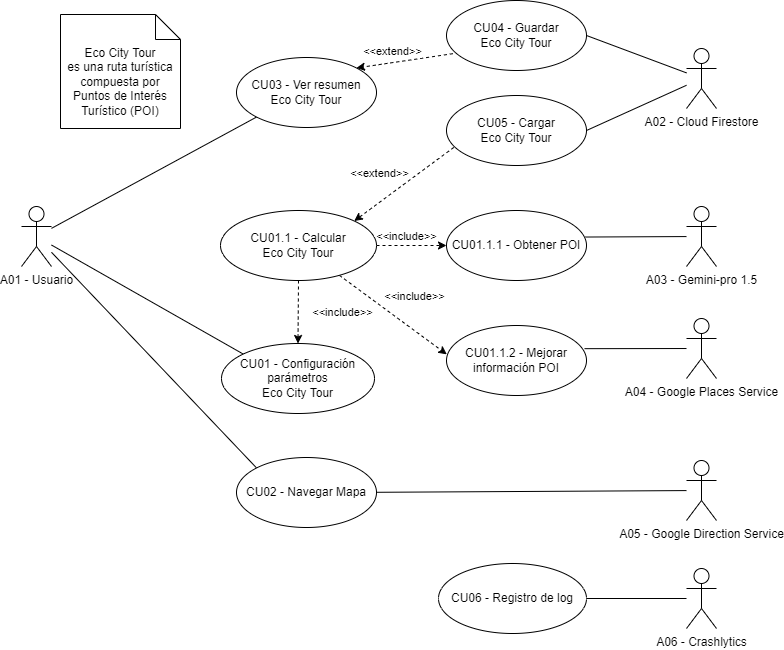
\includegraphics[scale=0.6]{casos-de-uso}
	\caption{Diagrama de casos de uso general de Eco City Tours}
	\label{fig:casos-de-uso}
\end{figure}


\subsection{CU01 - Configuración de parametros Eco City Tour}

\begin{table}[p]
	\centering
	\begin{tabularx}{\linewidth}{ p{0.21\columnwidth} p{0.71\columnwidth} }
		\toprule
		\textbf{CU01}    & \textbf{Configuración parámetros Eco City Tour} \\
		\toprule
		\textbf{Versión}              & 1.0    \\
		\textbf{Actor}                & A01 \\
		\textbf{Autor}                & \autor \\
		\textbf{Descripción}          & Configurar los parámetros necesarios para generar un Eco City Tour personalizado según las preferencias del usuario. \\
		\textbf{Precondición}         & El usuario accede a la pantalla de configuración. \\
		\textbf{Acciones}             &
		\begin{enumerate}
			\def\labelenumi{\arabic{enumi}.}
			\tightlist
			\item El usuario completa el formulario de preferencias, incluyendo el lugar, número de \acrshort{pdi}, medio de transporte y tiempo máximo.
		\end{enumerate}\\
		\textbf{Postcondición}        & Los parámetros quedan configurados y listos para generar la ruta. \\
		\textbf{Excepciones}          & 
		\begin{itemize}
			\tightlist
			\item El usuario no completa el formulario de configuración.
			\item Error en la carga de los datos de configuración.
		\end{itemize}\\
		\textbf{Importancia}          & Alta \\
		\bottomrule
	\end{tabularx}
	\caption{CU01 Configuración parámetros Eco City Tour}
\end{table}

\subsection{CU01.1 - Calcular Eco City Tour}
\begin{table}[p]
	\centering
	\begin{tabularx}{\linewidth}{ p{0.21\columnwidth} p{0.71\columnwidth} }
		\toprule
		\textbf{CU01.1}    & \textbf{Calcular Eco City Tour} \\
		\toprule
		\textbf{Versión}              & 1.0    \\
		\textbf{Actor}                & A03, A04, A05 \\
		\textbf{Autor}                & \autor \\
		\textbf{Descripción}          & Generar una ruta optimizada conectando los puntos de interés seleccionados en función de las preferencias del usuario. \\
		\textbf{Precondición}         & Los parámetros han sido configurados correctamente. \\
		\textbf{Acciones}             &
		\begin{enumerate}
			\def\labelenumi{\arabic{enumi}.}
			\tightlist
			\item El usuario confirma la configuración de preferencias.
			\item El sistema consulta un LLM para obtener \acrshort{pdi} basados en las preferencias del usuario.
			\item El sistema envía los \acrshort{pdi} a Google Places para obtener información mejorada.
			\item El sistema consulta un servicio de optimización de rutas para generar la ruta optimizada.
		\end{enumerate}\\
		\textbf{Postcondición}        & La ruta optimizada es calculada y lista para ser visualizada. \\
		\textbf{Excepciones}          & 
		\begin{itemize}
			\tightlist
			\item Fallo en la conexión con el LLM.
			\item Error en el servicio de optimización de rutas.
		\end{itemize}\\
		\textbf{Importancia}          & Alta \\
		\bottomrule
	\end{tabularx}
	\caption{CU01.1 Calcular Eco City Tour}
\end{table}

\subsection{CU02 - Navegar Mapa}


\begin{table}[p]
	\centering
	\begin{tabularx}{\linewidth}{ p{0.21\columnwidth} p{0.71\columnwidth} }
		\toprule
		\textbf{CU02}    & \textbf{Navegar Mapa} \\
		\toprule
		\textbf{Versión}              & 1.0    \\
		\textbf{Autor}                & \autor \\
		\textbf{Actor}                & A01 \\
		\textbf{Descripción}          & El usuario puede desplazarse y explorar el mapa interactivo de la aplicación. \\
		\textbf{Precondición}         & El mapa está visible. \\
		\textbf{Acciones}             &
		\begin{enumerate}
			\def\labelenumi{\arabic{enumi}.}
			\tightlist
			\item El usuario explora el mapa desplazándose y haciendo zoom.
		\end{enumerate}\\
		\textbf{Postcondición}        & El usuario navega por el mapa para observar los \acrshort{pdi} y la ruta. \\
		\textbf{Importancia}          & Media \\
		\bottomrule
	\end{tabularx}
	\caption{CU02 Navegar Mapa}
\end{table}


\begin{figure}[H]
	\centering
	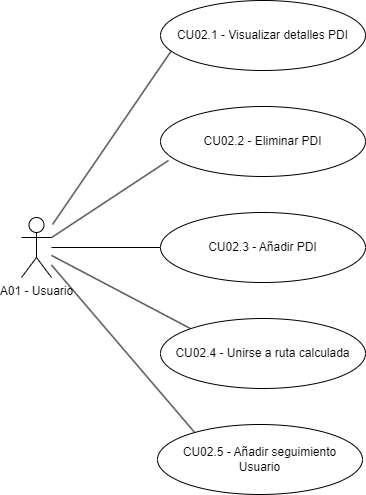
\includegraphics[scale=0.6]{CU02-Navegar-mapa}
	\caption{Diagrama de caso de uso CU02 - Navegar Mapa}
	\label{CU02-Navegar-mapa}
\end{figure}



\begin{table}[p]
	\centering
	\begin{tabularx}{\linewidth}{ p{0.21\columnwidth} p{0.71\columnwidth} }
		\toprule
		\textbf{CU02.1}    & \textbf{Visualizar detalles de \acrfull{pdi}} \\
		\toprule
		\textbf{Versión}              & 1.0    \\
		\textbf{Actor}                & A01 \\
		\textbf{Autor}                & \autor \\
		\textbf{Descripción}          & El usuario puede obtener información detallada sobre un punto de interés seleccionado en el mapa. \\
		\textbf{Precondición}         & La ruta y los puntos de interés están visibles en el mapa. \\
		\textbf{Acciones}             &
		\begin{enumerate}
			\def\labelenumi{\arabic{enumi}.}
			\tightlist
			\item El usuario selecciona un marcador de punto de interés en el mapa.
			\item El sistema muestra la información detallada del punto de interés.
		\end{enumerate}\\
		\textbf{Postcondición}        & La información detallada del punto de interés es visible para el usuario. \\
		\textbf{Excepciones}          & 
		\begin{itemize}
			\tightlist
			\item Fallo en la carga de información del \acrlong{pdi} debido a problemas de conectividad.
			\item Error en el servicio externo de obtención de información.
		\end{itemize}\\
		\textbf{Importancia}          & Alta \\
		\bottomrule
	\end{tabularx}
	\caption{CU02.1 Visualizar detalles de los \acrfull{pdi}}
\end{table}

\begin{table}[p]
	\centering
	\begin{tabularx}{\linewidth}{ p{0.21\columnwidth} p{0.71\columnwidth} }
		\toprule
		\textbf{CU02.2}    & \textbf{Eliminar \acrlong{pdi}} \\
		\toprule
		\textbf{Versión}              & 1.0    \\
		\textbf{Actor}                & A01, A05 \\
		\textbf{Autor}                & \autor \\
		\textbf{Descripción}          & El usuario puede eliminar puntos de interés de la ruta desde el mapa. \\
		\textbf{Precondición}         & La ruta ha sido generada y los puntos de interés están visibles en el mapa. \\
		\textbf{Acciones}             &
		\begin{enumerate}
			\def\labelenumi{\arabic{enumi}.}
			\tightlist
			\item El usuario selecciona un punto de interés en el mapa.
			\item El sistema elimina el punto de interés de la ruta.
			\item El sistema recalcula la ruta optimizada sin el punto eliminado.
		\end{enumerate}\\
		\textbf{Postcondición}        & La ruta es recalculada sin el punto de interés eliminado. \\
		\textbf{Excepciones}          & 
		\begin{itemize}
			\tightlist
			\item Error en el recálculo de la ruta.
			\item Problemas de conectividad al intentar actualizar la ruta.
		\end{itemize}\\
		\textbf{Importancia}          & Media \\
		\bottomrule
	\end{tabularx}
	\caption{CU02.2 Eliminar \acrlong{pdi}}
\end{table}

\begin{table}[p]
	\centering
	\begin{tabularx}{\linewidth}{ p{0.21\columnwidth} p{0.71\columnwidth} }
		\toprule
		\textbf{CU02.3}    & \textbf{Añadir \acrfull{pdi}} \\
		\toprule
		\textbf{Versión}              & 1.0    \\
		\textbf{Actor}                & A01 \\
		\textbf{Autor}                & \autor \\
		\textbf{Descripción}          & El usuario puede añadir manualmente un nuevo \acrshort{pdi} a la ruta introduciendo su nombre en la barra de búsqueda. \\
		\textbf{Precondición}         & La ruta ha sido generada previamente. \\
		\textbf{Acciones}             &
		\begin{enumerate}
			\def\labelenumi{\arabic{enumi}.}
			\tightlist
			\item El usuario introduce el nombre de un lugar en la barra de búsqueda.
			\item El sistema muestra el resultado de la búsqueda y el usuario lo selecciona para añadirlo.
			\item El sistema recalcula la ruta optimizada incluyendo el nuevo \acrlong{pdi}.
		\end{enumerate}\\
		\textbf{Postcondición}        & El nuevo lugar es añadido a la ruta, y la ruta optimizada es recalculada. \\
		\textbf{Excepciones}          & 
		\begin{itemize}
			\tightlist
			\item El lugar no se encuentra en el servicio de búsqueda.
			\item Fallo en el recalculo de la ruta.
		\end{itemize}\\
		\textbf{Importancia}          & Baja \\
		\bottomrule
	\end{tabularx}
	\caption{CU02.3 Añadir \acrfull{pdi}}
\end{table}

\begin{table}[p]
	\centering
	\begin{tabularx}{\linewidth}{ p{0.21\columnwidth} p{0.71\columnwidth} }
		\toprule
		\textbf{CU02.4}    & \textbf{Unirse a la ruta calculada} \\
		\toprule
		\textbf{Versión}              & 1.0    \\
		\textbf{Actor}                & A01 \\
		\textbf{Autor}                & \autor \\
		\textbf{Descripción}          & Permite al usuario unirse a una ruta previamente generada desde su ubicación actual. \\
		\textbf{Precondición}         & Una ruta ya ha sido generada y está activa. \\
		\textbf{Acciones}             &
		\begin{enumerate}
			\def\labelenumi{\arabic{enumi}.}
			\tightlist
			\item El usuario selecciona la opción para unirse a la ruta desde su ubicación actual.
			\item El sistema calcula la ruta más corta para conectar la ubicación actual del usuario con la ruta generada.
		\end{enumerate}\\
		\textbf{Postcondición}        & El usuario es guiado desde su ubicación actual hasta la ruta generada. \\
		\textbf{Excepciones}          & 
		\begin{itemize}
			\tightlist
			\item Error en el cálculo de la ruta de conexión.
			\item Problemas de conexión con el servicio de optimización de rutas.
		\end{itemize}\\
		\textbf{Importancia}          & Media \\
		\bottomrule
	\end{tabularx}
	\caption{CU02.4 Unirse a la ruta calculada}
\end{table}

\begin{table}[p]
	\centering
	\begin{tabularx}{\linewidth}{ p{0.21\columnwidth} p{0.71\columnwidth} }
		\toprule
		\textbf{CU02.5}    & \textbf{Añadir seguimiento del usuario} \\
		\toprule
		\textbf{Versión}              & 1.0    \\
		\textbf{Actor}                & A01 \\
		\textbf{Autor}                & \autor \\
		\textbf{Descripción}          & Permite al usuario activar o desactivar el seguimiento de su posición en tiempo real en el mapa. \\
		\textbf{Precondición}         & La aplicación tiene acceso a la ubicación del usuario. \\
		\textbf{Acciones}             &
		\begin{enumerate}
			\def\labelenumi{\arabic{enumi}.}
			\tightlist
			\item El usuario selecciona la opción de activar o desactivar el seguimiento de su ubicación en el mapa.
			\item El sistema ajusta el mapa para mostrar o dejar de mostrar el movimiento del usuario en tiempo real.
		\end{enumerate}\\
		\textbf{Postcondición}        & El mapa sigue o deja de seguir la posición del usuario en tiempo real. \\
		\textbf{Excepciones}          & 
		\begin{itemize}
			\tightlist
			\item Problemas de conexión con el GPS.
			\item Pérdida de señal GPS.
		\end{itemize}\\
		\textbf{Importancia}          & Baja \\
		\bottomrule
	\end{tabularx}
	\caption{CU02.5 Añadir seguimiento del usuario}
\end{table}


\subsection{CU03 - Ver resumen Eco City Tour}
\begin{table}[p]
	\centering
	\begin{tabularx}{\linewidth}{ p{0.21\columnwidth} p{0.71\columnwidth} }
		\toprule
		\textbf{CU03}    & \textbf{Ver resumen Eco City Tour} \\
		\toprule
		\textbf{Versión}              & 1.0    \\
		\textbf{Actor}                & A01 \\
		\textbf{Autor}                & \autor \\
		\textbf{Descripción}          & Muestra un resumen de la ruta generada, incluyendo la distancia, duración y medio de transporte. \\
		\textbf{Precondición}         & La ruta ha sido generada. \\
		\textbf{Acciones}             &
		\begin{enumerate}
			\def\labelenumi{\arabic{enumi}.}
			\tightlist
			\item El usuario accede a la pantalla de resumen.
			\item La aplicación muestra los detalles de la ruta, incluyendo distancia total, tiempo estimado y transporte elegido.
		\end{enumerate}\\
		\textbf{Postcondición}        & El resumen es visible para el usuario. \\
		\textbf{Excepciones}          & 
		\begin{itemize}
			\tightlist
			\item Error en la carga de los datos de la ruta.
		\end{itemize}\\
		\textbf{Importancia}          & Baja \\
		\bottomrule
	\end{tabularx}
	\caption{CU03 Ver resumen Eco City Tour}
\end{table}

\subsection{CU04 - Guardar Eco City Tour}
\begin{table}[p]
	\centering
	\begin{tabularx}{\linewidth}{ p{0.21\columnwidth} p{0.71\columnwidth} }
		\toprule
		\textbf{CU04}    & \textbf{Guardar Eco City Tour} \\
		\toprule
		\textbf{Versión}              & 1.0    \\
		\textbf{Actor}                & A01, A02 \\
		\textbf{Autor}                & \autor \\
		\textbf{Descripción}          & Permite al usuario guardar la ruta generada para acceder a ella en el futuro. \\
		\textbf{Precondición}         & La ruta ha sido generada. \\
		\textbf{Acciones}             &
		\begin{enumerate}
			\def\labelenumi{\arabic{enumi}.}
			\tightlist
			\item El usuario selecciona la opción de guardar la ruta.
		\end{enumerate}\\
		\textbf{Postcondición}        & La ruta queda guardada en el sistema. \\
		\textbf{Excepciones}          & 
		\begin{itemize}
			\tightlist
			\item Error en el guardado de la ruta.
			\item Problemas de conexión con la base de datos.
		\end{itemize}\\
		\textbf{Importancia}          & Media \\
		\bottomrule
	\end{tabularx}
	\caption{CU04 Guardar Eco City Tour}
\end{table}

\subsection{CU05 - Cargar Eco City Tour}
\begin{table}[p]
	\centering
	\begin{tabularx}{\linewidth}{ p{0.21\columnwidth} p{0.71\columnwidth} }
		\toprule
		\textbf{CU05}    & \textbf{Cargar Eco City Tour} \\
		\toprule
		\textbf{Versión}              & 1.0    \\
		\textbf{Actor}                & A01, A02 \\
		\textbf{Autor}                & \autor \\
		\textbf{Descripción}          & Permite al usuario cargar una ruta guardada previamente. \\
		\textbf{Precondición}         & El usuario ha guardado al menos una ruta. \\
		\textbf{Acciones}             &
		\begin{enumerate}
			\def\labelenumi{\arabic{enumi}.}
			\tightlist
			\item El usuario selecciona la opción de cargar una ruta guardada.
			\item El usuario selecciona un Eco City Tour guardado previamente que será cargado.
		\end{enumerate}\\
		\textbf{Postcondición}        & La ruta es cargada y visible en el mapa. \\
		\textbf{Excepciones}          & 
		\begin{itemize}
			\tightlist
			\item Error en la carga de la ruta guardada.
			\item Problemas de conexión con la base de datos.
		\end{itemize}\\
		\textbf{Importancia}          & Media \\
		\bottomrule
	\end{tabularx}
	\caption{CU05 Cargar Eco City Tour}
\end{table}

\subsection{CU06 - Registro de log}
\begin{table}[p]
	\centering
	\begin{tabularx}{\linewidth}{ p{0.21\columnwidth} p{0.71\columnwidth} }
		\toprule
		\textbf{CU06}    & \textbf{Registro de log} \\
		\toprule
		\textbf{Versión}              & 1.0    \\
		\textbf{Actor}                & A06 \\
		\textbf{Autor}                & \autor \\
		\textbf{Descripción}          & Registra los eventos y actividades del usuario en la aplicación para fines de monitorización y depuración. \\
		\textbf{Precondición}         & La aplicación está en funcionamiento. \\
		\textbf{Acciones}             &
		\begin{enumerate}
			\def\labelenumi{\arabic{enumi}.}
			\tightlist
			\item La aplicación registra automáticamente los eventos relevantes.
		\end{enumerate}\\
		\textbf{Postcondición}        & Los eventos quedan registrados en el sistema. \\
		\textbf{Excepciones}          & 
		\begin{itemize}
			\tightlist
			\item Error en la conexión con el sistema de registros.
			\item Fallo en la escritura de los eventos en el log.
		\end{itemize}\\
		\textbf{Importancia}          & Baja \\
		\bottomrule
	\end{tabularx}
	\caption{CU06 Registro de log}
\end{table}


\FloatBarrier


